\documentclass{article}
\usepackage[utf8]{inputenc}
\usepackage[legalpaper, portrait, margin=1in]{geometry}
\usepackage{amsmath}
\usepackage{pgfplots}
\usepackage{setspace}
\usepackage{indentfirst}
\usepackage{graphicx}
\graphicspath{ {./images/} }

\newtheorem{theorem}{Theorem}[section]
\newtheorem{definition}[theorem]{Definition}
\newtheorem{remark}[theorem]{Remark}
\newtheorem{postulate}[theorem]{Postulate}

\usepgfplotslibrary{external}
\tikzexternalize
\pgfplotsset{width=8cm,compat=1.9}
\setlength{\parindent}{20pt}


\title{MIT Research Supplement: A Collection of Mathematical Explorations}
\author{Edwin Trejo Balderas}
\date{November, 2022}

\begin{document}

\maketitle

\section{Introduction}
This document aims to offer a glimpse into the independent mathematical research/exploration I do in my free time and substantiate my deep love for mathematics. For brevity, I only present the major results of my explorations with some commentary on their motivation and/or applications.

\section{Powers and Modular Arithmetic}

(2.1) and (2.2) come from long-standing personal observations I made after thinking about the powers of 2 with reference to their use in computer binary. When generating numbers that consisted of consecutive 1's in binary and converting them to decimal, for example, I noticed how some of them were just shy of a multiple of 3. When I first learned how to do proofs by induction, these were the first two theorems I proved.

\begin{theorem}
    Any positive, even power of 2 is one more than a multiple of 3. 
    $$2^{2n}=3m+1;n,m\in\mbox{\textbf{Z}}^+$$
\end{theorem}

\begin{theorem}
    Any positive, odd power of 2 is one less than a multiple of 3. 
    $$2^{2n-1}=3m-1;n,m\in\mbox{\textbf{Z}}^+$$
\end{theorem}

(2.3) was an immediate observation I made after learning the basics of modular arithmetic and was also one of the first postulates I proved outside of school.

\begin{theorem}
    Let \mbox{p} be some positive integer, then the following holds:
    $$p^n\mod{(p+1)}=(-1)^n;p,n\in\mbox{\textbf{Z}}^+$$
\end{theorem}

(2.4) and (2.5) also come from observations which I made after I tried to extend the ideas in (2.1) and (2.2). I tried proving them by induction in a similar way I did (2.1) and (2.2), but ended up relying heavily on (2.3) instead.

\begin{theorem}
    Any positive, even power of some integer \mbox{p} is one more than a multiple of \mbox{p+1}. 
    $$p^{2n}=(p+1)m+1;p,n,m\in\mbox{\textbf{Z}}^+$$
\end{theorem}

\begin{theorem}
    Any positive, odd power of some integer \mbox{p} is one less than a multiple of \mbox{p+1}. 
    $$p^{2n-1}=(p+1)m-1;p,n,m\in\mbox{\textbf{Z}}^+$$
\end{theorem}

(2.6) came from the same observation as (2.1) and (2.2), but did not fully flesh itself out until I suddenly realized it is analagous to factorizations of the polynomial $z^n-1$, grabbed a pen and my notebook, and left the match of Tetris I was playing to frantically put everything down. 

\begin{theorem}
    For all positive integers, b, the following holds:
    $$b^n=(b-1)(b^0+b^1+\dots+b^{n-1})+1,;b,n\in\mbox{\textbf{Z}}^+$$
\end{theorem}

Examples where $b$ is a non-integer or negative also hold true, motivating future efforts at proving (2.7).

\begin{postulate}
    For all real numbers, b, the following holds:
    $$b^n=(b-1)(b^0+b^1+\dots+b^{n-1})+1,;b\in\mbox{\textbf{R}};b\in\mbox{\textbf{Z}}^+$$
\end{postulate}

\section{The Behavior of the Generalized Fibonacci Sequence}

For my IB Math Analysis Internal Assessment, I am studying the behavior of m-nacci sequences, a generalization of the fibonacci sequence.

\begin{definition}
An m-nacci sequence is a recursive sequence of the form:
$$F^{(m)}_n=F^{(m)}_{n-1}+F^{(m)}_{n-2}+\dots+F^{(m)}_{n-m}=\sum_{i=1}^m F^{(m)}_{n-i}$$
\end{definition}

\begin{remark}
    A system of equations can be derived from an m-nacci sequence:
    \begin{align*}
        F_n^{(m)} &= F^{(m)}_{n-1}+F^{(m)}_{n-2}+\dots+F^{(m)}_{n-m} \\ 
        F_{n-1}^{(m)} &= F_{n-1}^{(m)} \\ 
        F_{n-2}^{(m)} &= F_{n-2}^{(m)} \\
        &\vdots \\ 
        F_{n-m+1}^{(m)} &= F_{n-m+1}^{(m)}
    \end{align*}
    Which can be represented with a matrix equation:
    \begin{align*}
        \begin{bmatrix} 
            1 & 1 & 1 & \dots & 1 \\
            1 & 0 & 0 & \dots & 0 \\
            0 & 1 & 0 & \dots & 0 \\
            \vdots & & \ddots & \ddots  & \vdots \\ 
            0 & \dots & & 1 & 0
        \end{bmatrix}
        \begin{bmatrix} 
            F_{n-1} \\
            F_{n-2} \\
            F_{n-3} \\
            \vdots \\ 
            F_{n-m}
        \end{bmatrix} = 
        \begin{bmatrix} 
            F_{n} \\
            F_{n-1} \\
            F_{n-2} \\
            \vdots \\ 
            F_{n-m+1}
        \end{bmatrix}
    \end{align*}
\end{remark}

I use (3.3) in my Internal Assessment to serve as motivation for the construction of the characterisitc polynomial of generalized m-nacci sequences. The roots of the characteristic polynomial are later used in an algorithm to determine an explicit formula for an m-nacci sequence, similar to Binet's formula for the fibonacci sequence.

\begin{theorem}
    The characteristic polynomial of an $m\times m$ matrix of the form 
    \begin{align*}
    \begin{bmatrix} 
        1 & 1 & 1 & \dots & 1 \\
        1 & 0 & 0 & \dots & 0 \\
        0 & 1 & 0 & \dots & 0 \\
        \vdots & & \ddots & \ddots  & \vdots \\ 
        0 & \dots & & 1 & 0
    \end{bmatrix}
    \end{align*}
    is 
    $$t^m-t^{m-1}-t^{m-2}-\dots-t-1=t^m-\sum_{i=1}^m t^{m-i}$$
\end{theorem}

(3.4) came from an observation I made on the positive, real roots (which I will refer to as the 'leading root') of the characteristic polynomials from (3.3) which are used as bases for the explicit formulas mentioned above. Only the leading roots had a modulus greater than 1 and thus they become predominant as high indices of a sequence are determined. Furthermore, the leading roots approached but never reached 2, so I attempted and succeeded to prove that the limit the leading root approaches as the degree of an m-nacci sequence approaches infinity is 2.
For evidence, the explicit formulas for m-nacci sequences of degree 3, 4, and 5, determined by my algorithm, are given below with their leading roots in bold-face:
\begin{align*}
    F^{(3)}_n &= (0.0994)(\textbf{1.839})^n + (0.45 - 0.161i)(-0.42 + 0.606i)^n + (0.45 + 0.161i)(-0.420 - 0.606i)^n \\
    F^{(4)}_n &= (0.041)(\textbf{1.93})^n + (0.272 - 0.174i)(-0.0764 + 0.815i)^n + (0.272 + 0.174i)(-0.0764 - 0.815i)^n + \\ & (0.415)(-0.775)^n \\
    F^{(5)}_n &= (0.0183)(\textbf{1.97})^n + (0.171 - 0.152i)(0.195 + 0.849i)^n + (0.171 + 0.152i)(0.195 - 0.849i)^n + \\ & (0.32 - 0.0794i)(-0.678 + 0.459i)^n + (0.32 + 0.0794i)(-0.678 - 0.459i)^n
\end{align*}

\begin{theorem}
    The ratio between terms of an m-nacci sequence approaches the positive, real solution to the following expression:
    $$x+x^{-m}=2$$
    In other words, 
    $$\lim_{m \to \infty} \frac{F^{(m)}_n}{F^{(m)}_{n-1}}=\{x|x+x^{-m}=2\}$$
\end{theorem}

\section{The Reality of Complex Numbers and Their Conjugates}

I developed (4.1) to confirm that the explicit formulas for my Internal Assessment (such as $F^{(3)}_n$ from above), while containing complex exponential bases, would always return a real number. Notice that the terms that contain complex numbers in each explicit formula come in conjugate pairs.

\begin{theorem}
    The sum of the product of a set of complex numbers and the product of the set of conjugates is a real number:
    $$z_1z_2\dots z_n+\bar{z_1}\bar{z_2}\dots\bar{z_n}=\prod_{i=1}^n z_i+\prod_{i=1}^n \bar{z_i}=2R\cos{(\Phi)}$$
    Where
    $$z_j=a_j+ib_j;z_j\in\mbox{\textbf{C}};a_j,b_j\in\mbox{\textbf{R}}$$
    $$r_j=\sqrt{a_j^2+b_j^2};\theta_j=\tan^{-1}{\left(\frac{b_j}{a_j}\right)}$$
    $$R=r_1r_2\dots r_n=\prod_{i=1}^n r_i;\Phi=\theta_1+\theta_2+\dots+\theta_n=\sum_{i=1}^n$$
\end{theorem}

\section{Pascal's Simplex}

(5.2) was an extension upon a lesson from a discrete calculus course I took at the Georgia Governor's Honors Program. In the lesson, we used finite sums to derive formulas for figurate numbers such as the triangular, pentagonal, and tetrahedral numbers. I knew there are higher dimensional analogs of the triangle and tetrahderon and wanted to observe how their figurate numbers behaved.

\begin{definition}
    The falling exponent is defined as:
    \[x^{\underline{n}}=x(x-1)(x-2)\dots(x-n+1);x\in\mbox{\textbf{R}}^+,n\in\mbox{\textbf{Z}}^+\]
\end{definition}

\begin{theorem}
    The following sum:
    $$\sum_{x_2 = 0}^{x_1}\sum_{x_3 = 0}^{x_2}\dots\sum_{x_{m+1} = 0}^{x_m}1$$
    Evaluates to:
    $$\frac{{(x_1+m)}^{\underline{m}}}{m!}={{x_1+m} \choose {m}};x_i,m\in\mbox{\textbf{Z}}^+$$
\end{theorem}

Notice how using $m=3$ in (5.2) gives the formula for the tetrahedral numbers. In general, the expression gives the figurate number for the $(x+1)$th $m$-simplex.

(5.3) is an application of (5.2) I found after studying the multinomial theorem and its extensions on Pascal's Triangle with Pascal's Simplex. I am working on a program that constructs Pascal's Simplex and (5.3) has served useful in organizing how I will present the entries of high-dimensional simpleces.

\begin{theorem}
    The number of entries or multinomial coefficients in the r-th slice of pascal's m-simplex is given by 
    $$\sum_{x_2 = 0}^{r}\sum_{x_3 = 0}^{x_2}\dots\sum_{x_{m} = 0}^{x_{m-1}}1$$
    Which evaluates to:
    $$\frac{{(r+m-1)}^{\underline{m-1}}}{(m-1)!}={{r+m-1} \choose {m-1}};r,m\in\mbox{\textbf{Z}}^+$$
\end{theorem}

\section{A First Look into Real Analysis}
During the first semester of my senior year, I began self-studying real analysis and after playing with definitions and their implications, I proved the generalized triangle inequality using an induction technique similar to the one I used to prove (4.1).
\begin{theorem}
    For all $x_i\in\mbox{\textbf{R}}$, the following holds.
    \[|x_1+x_2+\dots+x_n|\leq |x_1|+|x_2|+\dots+|x_n|\Rightarrow |\sum_{i=1}^n x_i|\leq \sum_{i=1}^n |x_i|\]
\end{theorem}
Analysis is far more fun than internet communities would lead me to believe and has become one of my favorite fields of math. I am currently working on a proof that shows (6.1) holds for all complex numbers as well. 


\newpage

\section{Where it All Happens}
As I mentioned previously in the portfolio (and in the preface to (2.6)), this work takes place in a notebook that has at this point become a part of my daily life. So here I present, the book! The image below shows it open to rudimentary work leading to (3.3) (left) and a personal attempt at generalizing the representation of quadratic forms of any number of variables with matrices (right).

\begin{center}
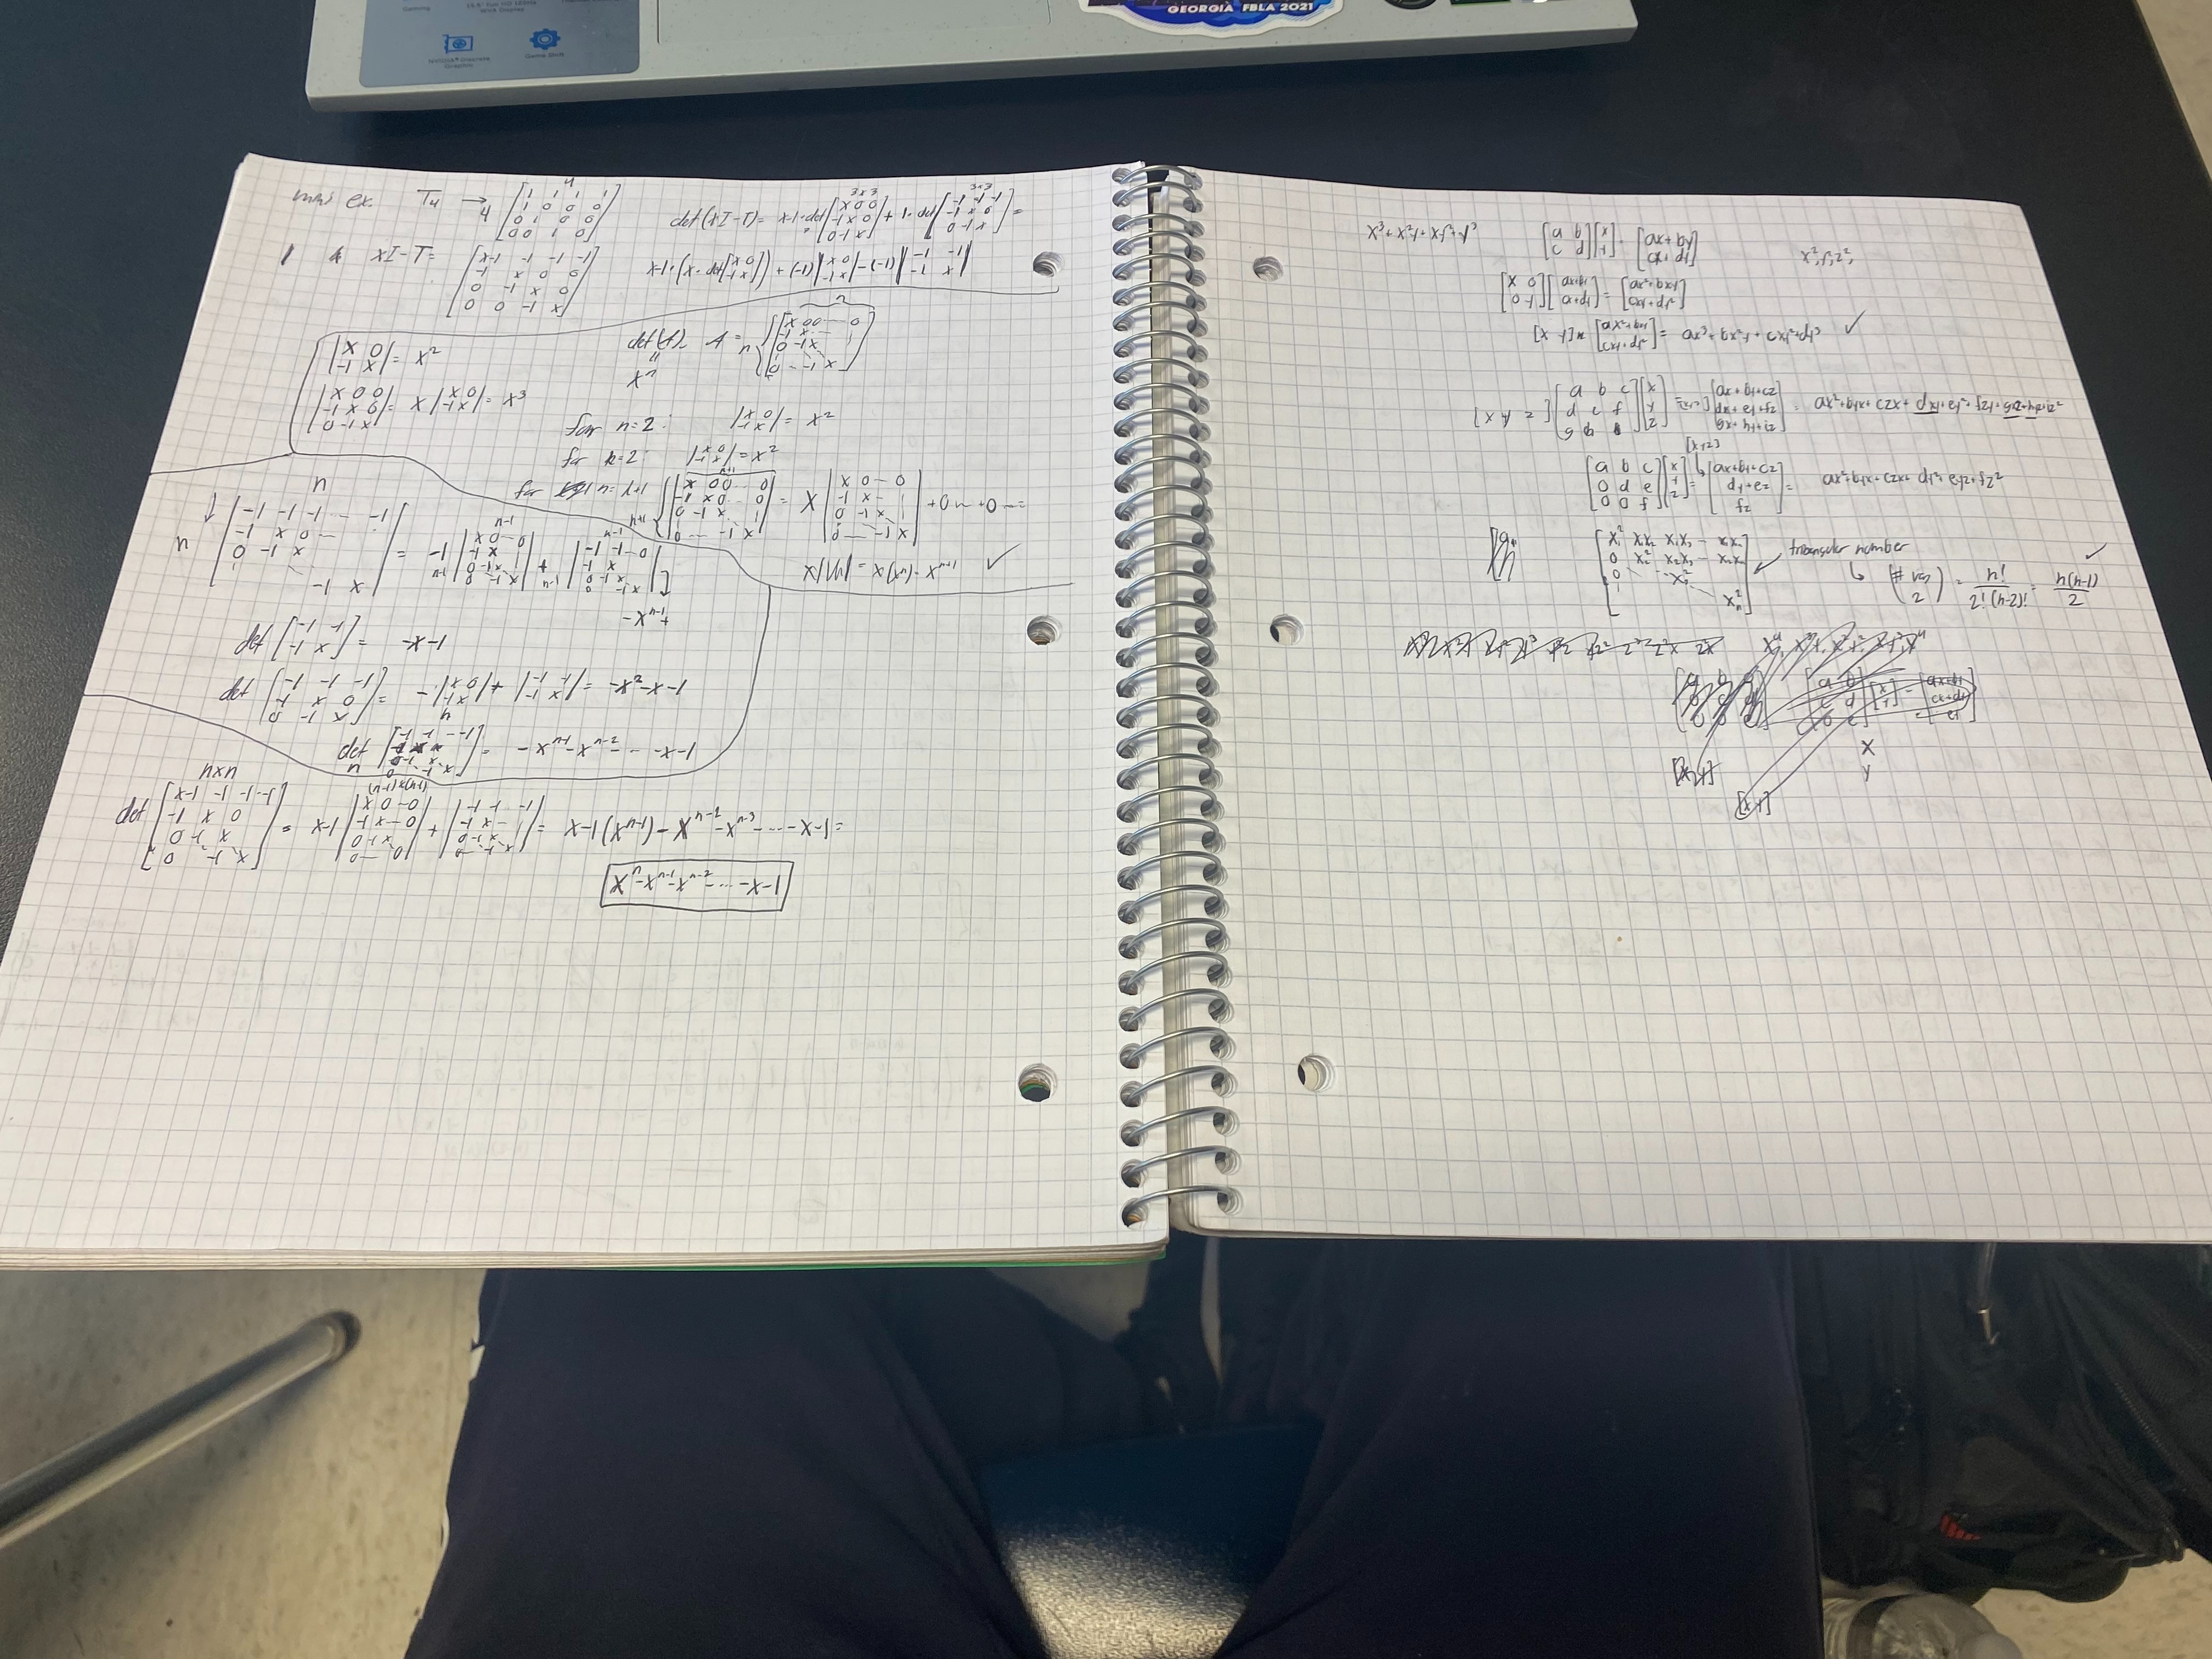
\includegraphics[scale=0.12]{image}
\end{center}

\end{document}